% ============================================================
% ［架空の記入例・提出不可］
% 症例数，数値，結果はすべて組版説明用である．引用文献だけは実在する．
% ============================================================
\begin{center}
  \UsamiFictionalExampleNotice
\end{center}

\AbstractSection{1．緒言}
腹部CTの多臓器領域分割は，臓器体積の定量化や手術支援の前処理として重要である．一方，3次元画像の輪郭付与には専門知識と時間を要し，単一施設では十分な症例数を確保しにくい．回転や弾性変形による従来のデータ拡張は実装が容易であるが，臓器間の位置関係や境界形状を破壊し，解剖学的に不自然な学習対を生成し得る．

本例では，臓器ラベルを条件とする潜在拡散モデルで腹部CTを合成し，解剖整合性を満たす画像・ラベル対だけを分割器の学習へ追加する．仮説は，学習更新回数を揃えた条件でも，品質選別と解剖正則化を併用すれば，実画像のみおよび選別なしの拡散拡張より患者単位の領域重複と境界精度が改善する，というものである．

\AbstractSection{2．関連研究}
U-Netは医用画像分割の代表的なエンコーダ・デコーダ構造であり\cite{ronneberger2015unet}，3D U-Netは疎な注釈から体積画像を学習する枠組みを示した\cite{cicek20163dunet}．本例では3D U-Netを分割器の基準モデルとする．

拡散モデルは，前向き過程で加えた雑音を逆過程で除去して画像分布を学習する\cite{ho2020ddpm}．潜在拡散モデルは，圧縮表現上で生成することで計算量と画像忠実度を両立させる\cite{rombach2022ldm}．ただし，医用画像拡張では画質だけでなく，条件ラベルと生成画像の対応，解剖学的妥当性，評価患者からの独立性を検証する必要がある．

\AbstractSection{3．問題設定}
門脈相腹部CT 84症例を対象とする架空設定とし，肝臓，脾臓，膵臓，左右腎，大動脈，門脈の7領域を分割する．全臓器を含まない撮像と強い体動を除外し，患者単位で学習50例，検証14例，評価20例へ固定する．同一患者のスライスを複数集合へ混入させず，評価集合はモデルと閾値を確定するまで使用しない．

\begin{center}
\small
\captionof{table}{データ分割と利用範囲（架空設定）．}
\label{tab:abstract-split}
\begin{tabularx}{\columnwidth}{l c X}
\toprule
集合 & 症例数 & 許可する用途 \\
\midrule
学習 & 50 & 生成器・分割器の学習，正規化統計 \\
検証 & 14 & 閾値，係数，停止時点，重み選択 \\
評価 & 20 & 固定済みモデルの最終評価だけ \\
\bottomrule
\end{tabularx}
\end{center}

表\ref{tab:abstract-split}の分割は前処理より先に患者IDで確定する．複数時点を持つ患者は全時点を同じ集合へ割り当て，撮像再構成や左右反転から派生した体積も元患者の集合を継承する．CT値の分位点，体幹cropの範囲，強度正規化統計は学習集合だけから求める．評価集合に対する除外は事前に定めた画質基準だけで行い，予測結果を見た後の症例除外を認めない．

注釈は医用画像の読影経験を持つ評価者が作成し，別の評価者が臓器欠損，左右取り違え，隣接臓器への漏出を確認する架空手順とした．不一致は予測結果を参照せず合議で確定し，修正履歴を固定する．学習前に注釈版を凍結し，評価後に修正が必要となった場合は主解析を置換せず，感度解析として分離する．

患者$i$のCT体積を$x_i$，ラベルを$y_i$，分割器を$f_\theta$とする．提案法は学習集合だけから合成対$(\tilde{x},\tilde{y})$を生成し，主要評価項目を7領域の患者内平均Dice係数，副次評価項目をHD95とする．

\AbstractSection{4．提案手法}
処理全体を図\ref{fig:abstract-pipeline}に示す．CTを等方性$1.5\,\mathrm{mm}$へ再標本化し，CT値を$[-150,250]$ HUへ制限する．潜在拡散モデルは実CTの圧縮表現に雑音を加え，変形した7臓器ラベルを条件として雑音を推定する．

再標本化ではCTへ三次線形補間，ラベルへ最近傍補間を用い，処理後の各臓器について連結成分数と体積変化率を記録する．crop後に臓器が欠けた体積は学習へ投入せず，元画像，変換行列，欠損臓器を監査表へ残す．入力方向はDICOM座標から統一し，左右反転の有無をラベル重心と画像方位の双方で照合する．

\begin{center}
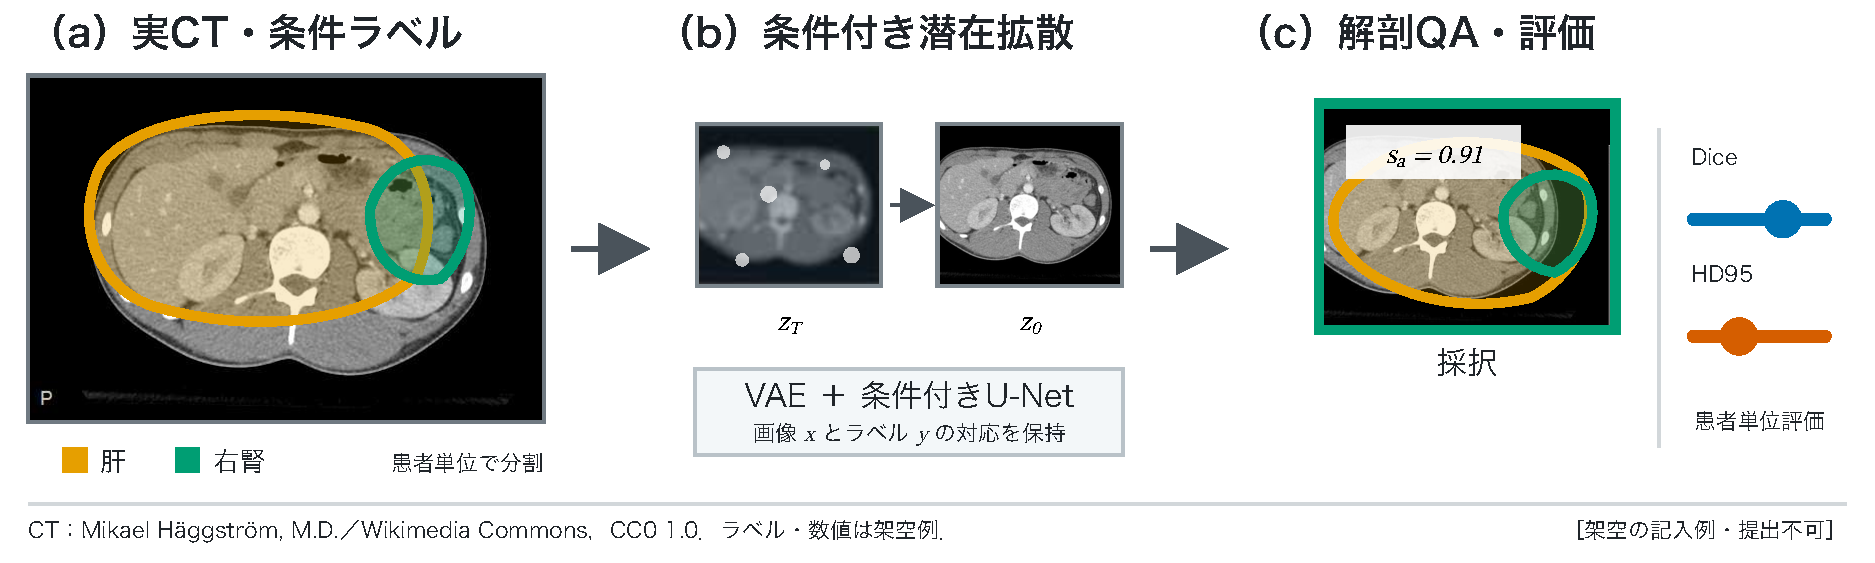
\includegraphics[width=0.68\columnwidth]{examples/figures/ct-diffusion-abstract.pdf}
\captionof{figure}{解剖構造保持拡散データ拡張の処理概要．}
\label{fig:abstract-pipeline}
\end{center}

生成候補は，臓器体積が学習分布の1--99パーセンタイル内，左右腎の重心順序が正常，排他的臓器間の重複率が0.5\%未満，固定した補助分割器と条件ラベルの平均Diceが0.75以上，という4条件で選別する．補助分割器は実画像50例だけで事前学習し，候補選別後は更新しない．評価患者の画像とラベルは生成にも選別にも用いない．

候補ごとに4条件の値を独立に保存し，最初に不合格となった理由だけでなく全条件の判定を残す．通過率を臓器別および元患者別に集計し，一部の解剖形状だけが過剰に採択されていないかを確認する．同一元患者から採択する候補数には上限を設け，ミニバッチ内で同一患者由来の実画像と合成画像が同時に現れないようにする．

潜在拡散モデルには，CTと7チャネルのone-hotラベルを体幹中心でcrop/padした$128\times192\times192$ voxelの3次元体積を入力する．自己符号化器の縮小率は各軸4，潜在チャネル数は8とし，条件ラベルは最近傍補間後に各U-Net解像度へ連結する．AdamW，初期学習率$1\times10^{-4}$，バッチサイズ1，勾配蓄積2で100,000更新し，検証損失が最小の重みを採用する．合成時は学習症例のラベルへ最大$\pm5\%$の拡大縮小と$\pm4\,\mathrm{mm}$の平行移動を加え，臓器がcrop境界で欠ける候補は生成前に除く．

最終分割器の損失を
\begin{equation}
  \mathcal{L}=\mathcal{L}_{\mathrm{Dice}}
  +\lambda_{\mathrm{ce}}\mathcal{L}_{\mathrm{CE}}
  +\lambda_{\mathrm{ana}}
    \bigl(\mathcal{L}_{\mathrm{vol}}+\mathcal{L}_{\mathrm{pos}}\bigr)
  \label{eq:abstract-loss}
\end{equation}
とする．式\eqref{eq:abstract-loss}の第3項は，予測臓器体積の外れと左右重心順序の反転を罰する．係数，生成枚数，停止時点は検証集合だけで決定する．実画像と合成画像の比率を1:1とし，全比較条件でミニバッチ数と更新回数を一致させる．

臓器$k$の物理体積を$v_{ik}$，予測体積を$\hat{v}_{ik}$とし，体積項を
\begin{equation}
  \mathcal{L}_{\mathrm{vol}}
  =\frac{1}{7B}\sum_{i=1}^{B}\sum_{k=1}^{7}
  \left|\log\frac{\hat{v}_{ik}+\epsilon}{v_{ik}+\epsilon}\right|
  \label{eq:abstract-volume}
\end{equation}
とする．式\eqref{eq:abstract-volume}では再標本化後のボクセル間隔を体積へ反映し，小臓器で分母が不安定になることを$\epsilon$で防ぐ．位置項は左右腎の重心座標にだけ適用し，正しい左右順序へ余分な拘束を加えない．これらは学習時の補助損失であり，評価時のDiceやHD95へ混ぜない．

分割器は5段の3D U-Netとし，初段チャネル数32，Instance Normalization，Leaky ReLUを用いる．学習時は前景を含むパッチを確率0.7で抽出し，AdamW，初期学習率$2\times10^{-4}$，weight decay $10^{-5}$で300 epoch学習する．検証Diceが30 epoch改善しない時点で停止し，推論時は50\%重複のsliding windowとガウス重み付き統合を用いる．幾何拡張条件では回転，拡大縮小，弾性変形だけを加え，拡散拡張条件との処理差を明確にする．

前処理，データ分割，候補の採否理由，乱数seed，最終checkpointを症例識別子とは別の実験台帳へ保存する．また，生成画像と学習画像の潜在特徴に基づく最近傍距離を算出し，上位5候補を目視監査する．これは記憶した症例の混入を完全に否定する検定ではないため，候補選別とは分けて記録する．

再現用記録には，入力体積とラベルのチェックサム，前処理設定，ライブラリ版，学習・推論コマンド，乱数seed，採択した重みのハッシュを含める．GPU演算の非決定性は消去できると仮定せず，同一設定を5乱数で独立に実行して変動を報告する．自動混合精度，勾配クリップ，欠損値処理の有無も条件間で固定し，実行途中の手作業による候補削除を禁止する．

匿名化は学習環境へ転送する前に行い，DICOMヘッダ，画像内へ焼き込まれた文字列，ファイル名の患者識別子を検査する．対応表は解析環境から分離し，生成画像には元症例IDではなく追跡用のランダムIDを付す．この手順は生成画像からの再同定不能性を保証するものではないため，外部共有の可否は最近傍監査と倫理審査の条件を含めて別途判断する．

% ここが物理的な1頁目と2頁目の境界である．
\AbstractPageBreak

\AbstractSection{5．実験・評価}
比較条件は，実画像のみ，幾何拡張，選別なしの拡散拡張，提案法の4条件とした．各条件を5乱数で学習し，患者ごとのDice係数とHD95を集計した．主要差の95\%信頼区間は評価患者を単位とする10,000回の対応付きブートストラップで求めた．表\ref{tab:abstract-results}を含むすべての症例数と結果は架空値である．

Diceは臓器ごとに算出した後，臓器体積に依存しない患者内macro平均とする．HD95は再標本化前の物理座標へ戻してmm単位で求め，予測が空の領域には評価体積の対角長を与える．表には5乱数の平均$\pm$標準偏差を示す一方，信頼区間は乱数ではなく患者間変動を反映する．評価集合では後処理，test-time augmentation，閾値の再調整を行わない．

主要比較は提案法と実画像のみの対応差とし，幾何拡張および選別なし拡散拡張との比較は副次解析とする．5乱数の予測は個別に保存し，同一患者内で乱数平均を求めてから患者を再標本化する．信頼区間が0をまたぐかだけで結論を二分せず，差の大きさ，患者間分布，悪化例数を併記する．空予測や推論失敗を欠測として削除せず，事前規則によるペナルティを適用する．

\begin{center}
\small
% 表題は表本体より上へ置く．
\captionof{table}{腹部CT多臓器分割の主要結果（架空値）．}
\label{tab:abstract-results}
\begin{tabular}{lcc}
\toprule
条件 & Dice$\uparrow$ & HD95 [mm]$\downarrow$ \\
\midrule
実画像のみ & $0.781\pm0.012$ & $12.8\pm1.4$ \\
幾何拡張 & $0.799\pm0.010$ & $11.6\pm1.2$ \\
拡散拡張 & $0.812\pm0.009$ & $10.9\pm1.0$ \\
提案法 & $\mathbf{0.826\pm0.008}$ & $\mathbf{9.7\pm0.9}$ \\
\bottomrule
\end{tabular}
\end{center}

提案法は実画像のみからDiceを0.045改善し，95\%信頼区間は$[0.031,0.058]$であった．HD95は$3.1\,\mathrm{mm}$低下し，差の信頼区間は$[-4.2,-2.0]\,\mathrm{mm}$であった．臓器別Diceの改善は膵臓で最大（$+0.071$），門脈で最小（$+0.006$）であり，細構造への効果は限定的であった．

\begin{center}
\small
\captionof{table}{臓器別Diceの例（架空値）．}
\label{tab:abstract-organs}
\begin{tabular}{lccc}
\toprule
臓器 & 実画像のみ & 提案法 & 差 \\
\midrule
肝臓 & 0.942 & 0.951 & $+0.009$ \\
脾臓 & 0.901 & 0.923 & $+0.022$ \\
膵臓 & 0.702 & 0.773 & $+0.071$ \\
門脈 & 0.684 & 0.690 & $+0.006$ \\
\bottomrule
\end{tabular}
\end{center}

表\ref{tab:abstract-organs}は効果の不均一性を示すための記入例であり，臓器ごとの4検定を独立な主要仮説として扱わない．主要推定量は患者内macro平均の対応差とし，ブートストラップでは患者を再標本化して同一患者内の臓器相関を保つ．臓器別値と失敗例は，平均改善の由来と限界を説明する副次解析として報告する．

患者単位では20例中17例でmacro Diceが改善し，1例は差が0.002未満，2例は低下した．低下例はいずれも門脈の造影が弱く，補助分割器の信頼度が高いにもかかわらず末梢枝が途切れた．一方，膵尾部の境界が不明瞭な症例では最大0.094改善した．平均値だけでなく改善・悪化症例を並べることで，提案法が全患者へ一様に効くわけではないことを確認した．

54候補中50例を採択し，左右関係の反転2例，臓器間重複1例，画像・条件不一致1例を除外した．ゲートと解剖項をともに除いた拡散拡張は表\ref{tab:abstract-results}の0.812であり，提案法から式\eqref{eq:abstract-loss}の解剖項だけを除くと0.819であった．合成数を実症例の0.5倍，1倍，2倍としたDiceはそれぞれ0.818，0.826，0.820であり，生成数の単純な増加では説明できなかった．

補助分割器の採択閾値を0.70，0.75，0.80と変えると，採択数は53，50，42例，Diceは0.821，0.826，0.824となった．緩い閾値では不整合候補が残り，厳しい閾値では症例多様性が減少した．また，$\lambda_{\mathrm{ana}}$を0，0.05，0.10，0.20としたDiceは0.819，0.823，0.826，0.817であり，過度な正則化は小臓器の個体差を抑制した．

頑健性解析では評価画像に合わせて再調整せず，固定済みモデルへ入力間隔の丸め，CT値窓の微小なずれ，crop余白の縮小を一因子ずつ加える．各摂動でDice，HD95，空予測率の変化を患者単位で報告する．臓器体積四分位，スライス厚，造影時刻による層別値は，優劣の確証ではなく失敗条件の探索として扱い，層別後の閾値変更を主解析へ戻さない．

計算負荷も分離して記録した．単一$80\,\mathrm{GB}$ GPUにおける架空値は，拡散モデル学習62.7 GPU h，実画像のみの分割器学習18.4 GPU h，提案法の分割器学習22.1 GPU hであった．生成処理は学習時だけに行うため，評価1症例の推論時間は基準法43秒，提案法44秒であった．性能差だけでなく，追加学習コストと運用時遅延を別指標として判断する必要がある．

\AbstractSection{6．考察}
同一更新回数の比較とアブレーションから，改善は合成画像数だけでなく，図\ref{fig:abstract-pipeline}の選別と解剖正則化に関連すると解釈できる．一方，単一施設84例の架空評価であり，装置，造影相，対象集団が異なる施設への一般化，臨床判断への寄与，門脈等の細構造への有効性は示していない．

品質閾値は学習分布に依存し，稀だが正常な解剖を除外する可能性がある．また，単一評価者の輪郭を正解とした設定では，観察者間変動を扱えない．実研究では外部施設評価，複数評価者による盲検確認，生成画像の最近傍監査を行い，倫理審査，匿名化，選択・除外基準，撮像条件を明記する必要がある．

さらに，補助分割器と最終分割器は類似した帰納バイアスを持つため，ゲート通過は独立な品質保証ではない．生成画像が既存症例を記憶していないことも，最近傍距離だけでは証明できない．外部利用時には独立モデルによる監査，生成候補の追跡可能性，実画像との類似度分布，失敗例を含むモデルカードを併記すべきである．

外部施設評価では，学習済み重み，前処理，閾値を凍結したまま施設単位のDice，HD95，空予測率を算出し，装置，スライス厚，造影相ごとの分布も併記する．外部データでの再学習や閾値調整を行う場合は，その結果を独立な適応実験として分離する．性能低下を施設間差だけへ帰属せず，撮像範囲，注釈規約，疾患構成の差を事前に定義した層別表で確認する必要がある．

\AbstractSection{7．結言}
少数症例下の腹部CT多臓器分割に対し，条件付き潜在拡散，品質ゲート，解剖正則化を組み合わせた．架空結果では患者単位のDiceとHD95が改善したが，細構造と外部施設での妥当性は未検証である．
